\documentclass[tikz,border=8pt]{standalone}
% Shared look for every TikZ diagram. Load with % Shared look for every TikZ diagram. Load with % Shared look for every TikZ diagram. Load with \input{../../tools/tikz-style.tex}
\usepackage[T1]{fontenc}
\usepackage{lmodern}
\renewcommand{\sfdefault}{lmr}  % diagrams use the same serif as the text
\usetikzlibrary{arrows.meta, positioning, shapes.geometric, calc, fit, backgrounds}
\definecolor{cblue}{HTML}{4C78A8}
\definecolor{corange}{HTML}{F58518}
\definecolor{cgreen}{HTML}{54A24B}
\definecolor{cred}{HTML}{E45756}
\definecolor{cpurple}{HTML}{B279A2}
\definecolor{cgrey}{HTML}{6B6B6B}
\tikzset{
  every picture/.style={font=\sffamily, line width=1.2pt},
  box/.style={draw=#1, fill=#1!12, rounded corners=4pt, align=center, inner sep=7pt, minimum height=1.1cm},
  box/.default=cgrey,
  arrow/.style={-{Stealth[length=3mm]}, draw=cgrey, line width=1.4pt},
  title/.style={font=\sffamily\bfseries\Large},
  note/.style={font=\sffamily\small, text=cgrey, align=center},
}
\AtBeginDocument{\hyphenpenalty=10000 \exhyphenpenalty=10000}

\usepackage[T1]{fontenc}
\usepackage{lmodern}
\renewcommand{\sfdefault}{lmr}  % diagrams use the same serif as the text
\usetikzlibrary{arrows.meta, positioning, shapes.geometric, calc, fit, backgrounds}
\definecolor{cblue}{HTML}{4C78A8}
\definecolor{corange}{HTML}{F58518}
\definecolor{cgreen}{HTML}{54A24B}
\definecolor{cred}{HTML}{E45756}
\definecolor{cpurple}{HTML}{B279A2}
\definecolor{cgrey}{HTML}{6B6B6B}
\tikzset{
  every picture/.style={font=\sffamily, line width=1.2pt},
  box/.style={draw=#1, fill=#1!12, rounded corners=4pt, align=center, inner sep=7pt, minimum height=1.1cm},
  box/.default=cgrey,
  arrow/.style={-{Stealth[length=3mm]}, draw=cgrey, line width=1.4pt},
  title/.style={font=\sffamily\bfseries\Large},
  note/.style={font=\sffamily\small, text=cgrey, align=center},
}
\AtBeginDocument{\hyphenpenalty=10000 \exhyphenpenalty=10000}

\usepackage[T1]{fontenc}
\usepackage{lmodern}
\renewcommand{\sfdefault}{lmr}  % diagrams use the same serif as the text
\usetikzlibrary{arrows.meta, positioning, shapes.geometric, calc, fit, backgrounds}
\definecolor{cblue}{HTML}{4C78A8}
\definecolor{corange}{HTML}{F58518}
\definecolor{cgreen}{HTML}{54A24B}
\definecolor{cred}{HTML}{E45756}
\definecolor{cpurple}{HTML}{B279A2}
\definecolor{cgrey}{HTML}{6B6B6B}
\tikzset{
  every picture/.style={font=\sffamily, line width=1.2pt},
  box/.style={draw=#1, fill=#1!12, rounded corners=4pt, align=center, inner sep=7pt, minimum height=1.1cm},
  box/.default=cgrey,
  arrow/.style={-{Stealth[length=3mm]}, draw=cgrey, line width=1.4pt},
  title/.style={font=\sffamily\bfseries\Large},
  note/.style={font=\sffamily\small, text=cgrey, align=center},
}
\AtBeginDocument{\hyphenpenalty=10000 \exhyphenpenalty=10000}

\begin{document}
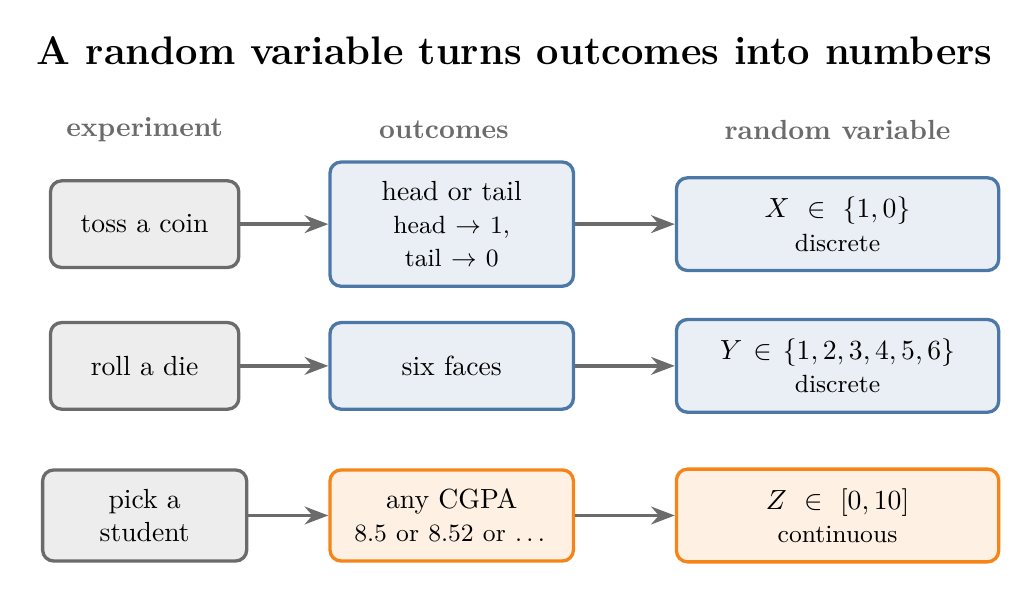
\begin{tikzpicture}[x=1cm, y=1cm]
  \node[title] at (5.5,4.6) {A random variable turns outcomes into numbers};
  \node[font=\sffamily\bfseries, text=cgrey] at (0.8,3.6) {experiment};
  \node[font=\sffamily\bfseries, text=cgrey] at (4.6,3.6) {outcomes};
  \node[font=\sffamily\bfseries, text=cgrey] at (9.6,3.6) {random variable};
  % coin
  \node[box=cgrey, text width=1.9cm] (coin) at (0.8,2.4) {toss a coin};
  \node[box=cblue, text width=2.6cm] (ht) at (4.7,2.4) {head or tail\\ \small head $\to$ 1, tail $\to$ 0};
  \node[box=cblue, text width=3.6cm] (x) at (9.6,2.4) {$X \in \{1, 0\}$\\ \small discrete};
  \draw[arrow] (coin) -- (ht); \draw[arrow] (ht) -- (x);
  % die
  \node[box=cgrey, text width=1.9cm] (die) at (0.8,0.6) {roll a die};
  \node[box=cblue, text width=2.6cm] (faces) at (4.7,0.6) {six faces};
  \node[box=cblue, text width=3.6cm] (y) at (9.6,0.6) {$Y \in \{1, 2, 3, 4, 5, 6\}$\\ \small discrete};
  \draw[arrow] (die) -- (faces); \draw[arrow] (faces) -- (y);
  % cgpa
  \node[box=cgrey, text width=2.1cm] (st) at (0.8,-1.3) {pick a student};
  \node[box=corange, text width=2.6cm] (cg) at (4.7,-1.3) {any CGPA\\ \small 8.5 or 8.52 or \dots};
  \node[box=corange, text width=3.6cm] (z) at (9.6,-1.3) {$Z \in [0, 10]$\\ \small continuous};
  \draw[arrow] (st) -- (cg); \draw[arrow] (cg) -- (z);
\end{tikzpicture}
\end{document}
